% Clase 01 -- Motivacion: los datos como corazon de la IA.
% COMPILA desde esta carpeta (para que ../../tema/ resuelva), DOS pasadas:
%   pdflatex -shell-escape -interaction=nonstopmode slides.tex
%   pdflatex -shell-escape -interaction=nonstopmode slides.tex
% Solo caracteres ASCII (acentos con comandos LaTeX: \'a \~n \c{c}).
\documentclass[aspectratio=169]{beamer}
% El tema ya carga inputenc, fontenc y babel (spanish si esta instalado).
% molina-tema.tex
% Tema Beamer institucional ITJMM / Tecnologico Superior de Jalisco.
% Se carga con % molina-tema.tex
% Tema Beamer institucional ITJMM / Tecnologico Superior de Jalisco.
% Se carga con % molina-tema.tex
% Tema Beamer institucional ITJMM / Tecnologico Superior de Jalisco.
% Se carga con \input{../../tema/molina-tema.tex} desde slides.tex,
% que vive en clases/XX-tema/. COMPILAR SIEMPRE desde la carpeta de la
% clase para que las rutas relativas (../../tema/) resuelvan.
%
% Provee:
%   - Paleta institucional (molTeal, molNaranja, molAmarillo, molMorado).
%   - Franja vectorial de colores (\molinaBanner) en portada y separadores.
%   - Ambos logos (\molinaLogos) en portada y separadores.
%   - Slides de contenido limpias: titulo con regla teal + footline con
%     logo pequeno, titulo corto y numero de slide.
% Solo caracteres ASCII.

% Codificacion e idioma. Spanish de babel solo si esta instalado
% (texlive-lang-spanish); si no, cae a english para no romper el build.
\usepackage[utf8]{inputenc}
\usepackage[T1]{fontenc}
\IfFileExists{spanish.ldf}%
  {\usepackage[spanish]{babel}}%
  {\usepackage[english]{babel}}

\usepackage{tikz}
\usetikzlibrary{calc}
\usepackage{listings}

% --- Paleta (muestreada del master institucional) -----------------------
\definecolor{molTeal}{HTML}{0094A2}
\definecolor{molTealLt}{HTML}{00B0B5}
\definecolor{molNaranja}{HTML}{FE730C}
\definecolor{molRojo}{HTML}{FF5A0C}
\definecolor{molAmarillo}{HTML}{FEB200}
\definecolor{molMorado}{HTML}{532587}
\definecolor{molOro}{HTML}{B8860B}
\definecolor{molAzul}{HTML}{1F4E9B}

% --- Donde buscar logos y figuras ---------------------------------------
\graphicspath{{../../tema/}{figuras/}{datos/}}

% --- Colores de elementos Beamer ----------------------------------------
\setbeamercolor{structure}{fg=molTeal}
\setbeamercolor{frametitle}{fg=molTeal}
\setbeamercolor{title}{fg=molMorado}
\setbeamercolor{itemize item}{fg=molNaranja}
\setbeamercolor{itemize subitem}{fg=molTeal}
\setbeamercolor{block title}{bg=molTeal,fg=white}
\setbeamercolor{block body}{bg=molTeal!8,fg=black}
\setbeamertemplate{itemize items}[circle]
\setbeamertemplate{navigation symbols}{}

% --- Franja superior vectorial (formas angulares) -----------------------
% Anclada a las esquinas de la pagina; no depende del ancho exacto.
\newcommand{\molinaBanner}{%
  \begin{tikzpicture}[remember picture,overlay]
    \coordinate (O) at (current page.north west);
    \coordinate (E) at (current page.north east);
    % Bloque teal principal (izquierda)
    \fill[molTeal]    ($(O)+(0,0)$) -- ($(O)+(3.7,0)$) -- ($(O)+(3.1,-0.55)$) -- ($(O)+(0,-0.55)$) -- cycle;
    % Acento teal claro
    \fill[molTealLt]  ($(O)+(3.7,0)$) -- ($(O)+(4.5,0)$) -- ($(O)+(3.9,-0.55)$) -- ($(O)+(3.1,-0.55)$) -- cycle;
    % Muesca morada bajo el teal
    \fill[molMorado]  ($(O)+(0,-0.55)$) -- ($(O)+(0.75,-0.55)$) -- ($(O)+(0,-1.05)$) -- cycle;
    % Bloque naranja (centro-derecha)
    \fill[molNaranja] ($(E)+(-4.5,0)$) -- ($(E)+(-7.3,0)$) -- ($(E)+(-7.9,-0.55)$) -- ($(E)+(-5.1,-0.55)$) -- cycle;
    % Bloque rojo-naranja
    \fill[molRojo]    ($(E)+(-2.9,0)$) -- ($(E)+(-4.5,0)$) -- ($(E)+(-5.1,-0.55)$) -- ($(E)+(-3.5,-0.55)$) -- cycle;
    % Bloque amarillo (derecha)
    \fill[molAmarillo]($(E)+(0,0)$) -- ($(E)+(-2.9,0)$) -- ($(E)+(-3.5,-0.55)$) -- ($(E)+(0,-0.55)$) -- cycle;
  \end{tikzpicture}%
}

% --- Logos institucionales en el pie ------------------------------------
\newcommand{\molinaLogos}{%
  \begin{tikzpicture}[remember picture,overlay]
    \node[anchor=south west, inner sep=0pt]
      at ($(current page.south west)+(0.7cm,0.45cm)$)
      {
\includegraphics[height=1.05cm]{logo_mario_molina}};
    \node[anchor=south east, inner sep=0pt]
      at ($(current page.south east)+(-0.7cm,0.55cm)$)
      {
\includegraphics[height=0.85cm]{logo_TSJ}};
  \end{tikzpicture}%
}

% --- Portada -------------------------------------------------------------
% Usar dentro de \begin{frame}[plain]\titlepage\end{frame}
\setbeamertemplate{title page}{%
  \molinaBanner%
  \vfill
  \begin{center}
    {\usebeamercolor[fg]{title}\Large\bfseries\inserttitle\par}
    \vspace{0.4em}
    {\color{molTeal}\large\insertsubtitle\par}
    \vspace{1.6em}
    {\small\insertauthor\par}
    {\scriptsize\insertdate\par}
  \end{center}
  \vfill\vspace{1.0cm}%
  \molinaLogos%
}

% --- Separador de seccion -----------------------------------------------
\setbeamertemplate{section page}{%
  \molinaBanner%
  \vfill
  \begin{center}
    {\color{molTeal}\footnotesize SECCION\par}
    \vspace{0.3em}
    {\color{molMorado}\Large\bfseries\insertsectionhead\par}
  \end{center}
  \vfill\vspace{1.0cm}%
  \molinaLogos%
}
\AtBeginSection[]{%
  \begin{frame}[plain]\sectionpage\end{frame}%
}

% --- Frame de contenido: titulo con regla teal --------------------------
\setbeamertemplate{headline}{}
\setbeamertemplate{frametitle}{%
  \vspace*{0.4em}\hspace*{0.2em}%
  {\usebeamercolor[fg]{frametitle}\bfseries\insertframetitle}\par
  \vspace*{0.12em}\hspace*{0.2em}%
  {\color{molTeal}\rule{0.985\paperwidth}{1.2pt}}%
}

% --- Pie de slides de contenido -----------------------------------------
\setbeamertemplate{footline}{%
  \leavevmode%
  \hbox{%
    \begin{beamercolorbox}[wd=.22\paperwidth,ht=2.6ex,dp=1.1ex,leftskip=.4em]{}%
      \raisebox{-0.2ex}{
\includegraphics[height=1.7ex]{logo_mario_molina}}%
    \end{beamercolorbox}%
    \begin{beamercolorbox}[wd=.56\paperwidth,ht=2.6ex,dp=1.1ex,center]{}%
      {\scriptsize\color{molTeal}\insertshorttitle}%
    \end{beamercolorbox}%
    \begin{beamercolorbox}[wd=.22\paperwidth,ht=2.6ex,dp=1.1ex,rightskip=.4em]{}%
      \hfill{\scriptsize\color{molTeal}\insertframenumber}%
    \end{beamercolorbox}%
  }\vskip2pt%
}

% --- Estilo para bloques de codigo (listings) ---------------------------
\lstset{
  basicstyle=\ttfamily\small,
  keywordstyle=\color{molMorado}\bfseries,
  commentstyle=\color{molTeal}\itshape,
  stringstyle=\color{molNaranja},
  numberstyle=\tiny\color{gray},
  frame=single,
  rulecolor=\color{molTeal},
  backgroundcolor=\color{molTeal!5},
  breaklines=true,
  showstringspaces=false,
  tabsize=4,
  language=Python
}
 desde slides.tex,
% que vive en clases/XX-tema/. COMPILAR SIEMPRE desde la carpeta de la
% clase para que las rutas relativas (../../tema/) resuelvan.
%
% Provee:
%   - Paleta institucional (molTeal, molNaranja, molAmarillo, molMorado).
%   - Franja vectorial de colores (\molinaBanner) en portada y separadores.
%   - Ambos logos (\molinaLogos) en portada y separadores.
%   - Slides de contenido limpias: titulo con regla teal + footline con
%     logo pequeno, titulo corto y numero de slide.
% Solo caracteres ASCII.

% Codificacion e idioma. Spanish de babel solo si esta instalado
% (texlive-lang-spanish); si no, cae a english para no romper el build.
\usepackage[utf8]{inputenc}
\usepackage[T1]{fontenc}
\IfFileExists{spanish.ldf}%
  {\usepackage[spanish]{babel}}%
  {\usepackage[english]{babel}}

\usepackage{tikz}
\usetikzlibrary{calc}
\usepackage{listings}

% --- Paleta (muestreada del master institucional) -----------------------
\definecolor{molTeal}{HTML}{0094A2}
\definecolor{molTealLt}{HTML}{00B0B5}
\definecolor{molNaranja}{HTML}{FE730C}
\definecolor{molRojo}{HTML}{FF5A0C}
\definecolor{molAmarillo}{HTML}{FEB200}
\definecolor{molMorado}{HTML}{532587}
\definecolor{molOro}{HTML}{B8860B}
\definecolor{molAzul}{HTML}{1F4E9B}

% --- Donde buscar logos y figuras ---------------------------------------
\graphicspath{{../../tema/}{figuras/}{datos/}}

% --- Colores de elementos Beamer ----------------------------------------
\setbeamercolor{structure}{fg=molTeal}
\setbeamercolor{frametitle}{fg=molTeal}
\setbeamercolor{title}{fg=molMorado}
\setbeamercolor{itemize item}{fg=molNaranja}
\setbeamercolor{itemize subitem}{fg=molTeal}
\setbeamercolor{block title}{bg=molTeal,fg=white}
\setbeamercolor{block body}{bg=molTeal!8,fg=black}
\setbeamertemplate{itemize items}[circle]
\setbeamertemplate{navigation symbols}{}

% --- Franja superior vectorial (formas angulares) -----------------------
% Anclada a las esquinas de la pagina; no depende del ancho exacto.
\newcommand{\molinaBanner}{%
  \begin{tikzpicture}[remember picture,overlay]
    \coordinate (O) at (current page.north west);
    \coordinate (E) at (current page.north east);
    % Bloque teal principal (izquierda)
    \fill[molTeal]    ($(O)+(0,0)$) -- ($(O)+(3.7,0)$) -- ($(O)+(3.1,-0.55)$) -- ($(O)+(0,-0.55)$) -- cycle;
    % Acento teal claro
    \fill[molTealLt]  ($(O)+(3.7,0)$) -- ($(O)+(4.5,0)$) -- ($(O)+(3.9,-0.55)$) -- ($(O)+(3.1,-0.55)$) -- cycle;
    % Muesca morada bajo el teal
    \fill[molMorado]  ($(O)+(0,-0.55)$) -- ($(O)+(0.75,-0.55)$) -- ($(O)+(0,-1.05)$) -- cycle;
    % Bloque naranja (centro-derecha)
    \fill[molNaranja] ($(E)+(-4.5,0)$) -- ($(E)+(-7.3,0)$) -- ($(E)+(-7.9,-0.55)$) -- ($(E)+(-5.1,-0.55)$) -- cycle;
    % Bloque rojo-naranja
    \fill[molRojo]    ($(E)+(-2.9,0)$) -- ($(E)+(-4.5,0)$) -- ($(E)+(-5.1,-0.55)$) -- ($(E)+(-3.5,-0.55)$) -- cycle;
    % Bloque amarillo (derecha)
    \fill[molAmarillo]($(E)+(0,0)$) -- ($(E)+(-2.9,0)$) -- ($(E)+(-3.5,-0.55)$) -- ($(E)+(0,-0.55)$) -- cycle;
  \end{tikzpicture}%
}

% --- Logos institucionales en el pie ------------------------------------
\newcommand{\molinaLogos}{%
  \begin{tikzpicture}[remember picture,overlay]
    \node[anchor=south west, inner sep=0pt]
      at ($(current page.south west)+(0.7cm,0.45cm)$)
      {
\includegraphics[height=1.05cm]{logo_mario_molina}};
    \node[anchor=south east, inner sep=0pt]
      at ($(current page.south east)+(-0.7cm,0.55cm)$)
      {
\includegraphics[height=0.85cm]{logo_TSJ}};
  \end{tikzpicture}%
}

% --- Portada -------------------------------------------------------------
% Usar dentro de \begin{frame}[plain]\titlepage\end{frame}
\setbeamertemplate{title page}{%
  \molinaBanner%
  \vfill
  \begin{center}
    {\usebeamercolor[fg]{title}\Large\bfseries\inserttitle\par}
    \vspace{0.4em}
    {\color{molTeal}\large\insertsubtitle\par}
    \vspace{1.6em}
    {\small\insertauthor\par}
    {\scriptsize\insertdate\par}
  \end{center}
  \vfill\vspace{1.0cm}%
  \molinaLogos%
}

% --- Separador de seccion -----------------------------------------------
\setbeamertemplate{section page}{%
  \molinaBanner%
  \vfill
  \begin{center}
    {\color{molTeal}\footnotesize SECCION\par}
    \vspace{0.3em}
    {\color{molMorado}\Large\bfseries\insertsectionhead\par}
  \end{center}
  \vfill\vspace{1.0cm}%
  \molinaLogos%
}
\AtBeginSection[]{%
  \begin{frame}[plain]\sectionpage\end{frame}%
}

% --- Frame de contenido: titulo con regla teal --------------------------
\setbeamertemplate{headline}{}
\setbeamertemplate{frametitle}{%
  \vspace*{0.4em}\hspace*{0.2em}%
  {\usebeamercolor[fg]{frametitle}\bfseries\insertframetitle}\par
  \vspace*{0.12em}\hspace*{0.2em}%
  {\color{molTeal}\rule{0.985\paperwidth}{1.2pt}}%
}

% --- Pie de slides de contenido -----------------------------------------
\setbeamertemplate{footline}{%
  \leavevmode%
  \hbox{%
    \begin{beamercolorbox}[wd=.22\paperwidth,ht=2.6ex,dp=1.1ex,leftskip=.4em]{}%
      \raisebox{-0.2ex}{
\includegraphics[height=1.7ex]{logo_mario_molina}}%
    \end{beamercolorbox}%
    \begin{beamercolorbox}[wd=.56\paperwidth,ht=2.6ex,dp=1.1ex,center]{}%
      {\scriptsize\color{molTeal}\insertshorttitle}%
    \end{beamercolorbox}%
    \begin{beamercolorbox}[wd=.22\paperwidth,ht=2.6ex,dp=1.1ex,rightskip=.4em]{}%
      \hfill{\scriptsize\color{molTeal}\insertframenumber}%
    \end{beamercolorbox}%
  }\vskip2pt%
}

% --- Estilo para bloques de codigo (listings) ---------------------------
\lstset{
  basicstyle=\ttfamily\small,
  keywordstyle=\color{molMorado}\bfseries,
  commentstyle=\color{molTeal}\itshape,
  stringstyle=\color{molNaranja},
  numberstyle=\tiny\color{gray},
  frame=single,
  rulecolor=\color{molTeal},
  backgroundcolor=\color{molTeal!5},
  breaklines=true,
  showstringspaces=false,
  tabsize=4,
  language=Python
}
 desde slides.tex,
% que vive en clases/XX-tema/. COMPILAR SIEMPRE desde la carpeta de la
% clase para que las rutas relativas (../../tema/) resuelvan.
%
% Provee:
%   - Paleta institucional (molTeal, molNaranja, molAmarillo, molMorado).
%   - Franja vectorial de colores (\molinaBanner) en portada y separadores.
%   - Ambos logos (\molinaLogos) en portada y separadores.
%   - Slides de contenido limpias: titulo con regla teal + footline con
%     logo pequeno, titulo corto y numero de slide.
% Solo caracteres ASCII.

% Codificacion e idioma. Spanish de babel solo si esta instalado
% (texlive-lang-spanish); si no, cae a english para no romper el build.
\usepackage[utf8]{inputenc}
\usepackage[T1]{fontenc}
\IfFileExists{spanish.ldf}%
  {\usepackage[spanish]{babel}}%
  {\usepackage[english]{babel}}

\usepackage{tikz}
\usetikzlibrary{calc}
\usepackage{listings}

% --- Paleta (muestreada del master institucional) -----------------------
\definecolor{molTeal}{HTML}{0094A2}
\definecolor{molTealLt}{HTML}{00B0B5}
\definecolor{molNaranja}{HTML}{FE730C}
\definecolor{molRojo}{HTML}{FF5A0C}
\definecolor{molAmarillo}{HTML}{FEB200}
\definecolor{molMorado}{HTML}{532587}
\definecolor{molOro}{HTML}{B8860B}
\definecolor{molAzul}{HTML}{1F4E9B}

% --- Donde buscar logos y figuras ---------------------------------------
\graphicspath{{../../tema/}{figuras/}{datos/}}

% --- Colores de elementos Beamer ----------------------------------------
\setbeamercolor{structure}{fg=molTeal}
\setbeamercolor{frametitle}{fg=molTeal}
\setbeamercolor{title}{fg=molMorado}
\setbeamercolor{itemize item}{fg=molNaranja}
\setbeamercolor{itemize subitem}{fg=molTeal}
\setbeamercolor{block title}{bg=molTeal,fg=white}
\setbeamercolor{block body}{bg=molTeal!8,fg=black}
\setbeamertemplate{itemize items}[circle]
\setbeamertemplate{navigation symbols}{}

% --- Franja superior vectorial (formas angulares) -----------------------
% Anclada a las esquinas de la pagina; no depende del ancho exacto.
\newcommand{\molinaBanner}{%
  \begin{tikzpicture}[remember picture,overlay]
    \coordinate (O) at (current page.north west);
    \coordinate (E) at (current page.north east);
    % Bloque teal principal (izquierda)
    \fill[molTeal]    ($(O)+(0,0)$) -- ($(O)+(3.7,0)$) -- ($(O)+(3.1,-0.55)$) -- ($(O)+(0,-0.55)$) -- cycle;
    % Acento teal claro
    \fill[molTealLt]  ($(O)+(3.7,0)$) -- ($(O)+(4.5,0)$) -- ($(O)+(3.9,-0.55)$) -- ($(O)+(3.1,-0.55)$) -- cycle;
    % Muesca morada bajo el teal
    \fill[molMorado]  ($(O)+(0,-0.55)$) -- ($(O)+(0.75,-0.55)$) -- ($(O)+(0,-1.05)$) -- cycle;
    % Bloque naranja (centro-derecha)
    \fill[molNaranja] ($(E)+(-4.5,0)$) -- ($(E)+(-7.3,0)$) -- ($(E)+(-7.9,-0.55)$) -- ($(E)+(-5.1,-0.55)$) -- cycle;
    % Bloque rojo-naranja
    \fill[molRojo]    ($(E)+(-2.9,0)$) -- ($(E)+(-4.5,0)$) -- ($(E)+(-5.1,-0.55)$) -- ($(E)+(-3.5,-0.55)$) -- cycle;
    % Bloque amarillo (derecha)
    \fill[molAmarillo]($(E)+(0,0)$) -- ($(E)+(-2.9,0)$) -- ($(E)+(-3.5,-0.55)$) -- ($(E)+(0,-0.55)$) -- cycle;
  \end{tikzpicture}%
}

% --- Logos institucionales en el pie ------------------------------------
\newcommand{\molinaLogos}{%
  \begin{tikzpicture}[remember picture,overlay]
    \node[anchor=south west, inner sep=0pt]
      at ($(current page.south west)+(0.7cm,0.45cm)$)
      {
\includegraphics[height=1.05cm]{logo_mario_molina}};
    \node[anchor=south east, inner sep=0pt]
      at ($(current page.south east)+(-0.7cm,0.55cm)$)
      {
\includegraphics[height=0.85cm]{logo_TSJ}};
  \end{tikzpicture}%
}

% --- Portada -------------------------------------------------------------
% Usar dentro de \begin{frame}[plain]\titlepage\end{frame}
\setbeamertemplate{title page}{%
  \molinaBanner%
  \vfill
  \begin{center}
    {\usebeamercolor[fg]{title}\Large\bfseries\inserttitle\par}
    \vspace{0.4em}
    {\color{molTeal}\large\insertsubtitle\par}
    \vspace{1.6em}
    {\small\insertauthor\par}
    {\scriptsize\insertdate\par}
  \end{center}
  \vfill\vspace{1.0cm}%
  \molinaLogos%
}

% --- Separador de seccion -----------------------------------------------
\setbeamertemplate{section page}{%
  \molinaBanner%
  \vfill
  \begin{center}
    {\color{molTeal}\footnotesize SECCION\par}
    \vspace{0.3em}
    {\color{molMorado}\Large\bfseries\insertsectionhead\par}
  \end{center}
  \vfill\vspace{1.0cm}%
  \molinaLogos%
}
\AtBeginSection[]{%
  \begin{frame}[plain]\sectionpage\end{frame}%
}

% --- Frame de contenido: titulo con regla teal --------------------------
\setbeamertemplate{headline}{}
\setbeamertemplate{frametitle}{%
  \vspace*{0.4em}\hspace*{0.2em}%
  {\usebeamercolor[fg]{frametitle}\bfseries\insertframetitle}\par
  \vspace*{0.12em}\hspace*{0.2em}%
  {\color{molTeal}\rule{0.985\paperwidth}{1.2pt}}%
}

% --- Pie de slides de contenido -----------------------------------------
\setbeamertemplate{footline}{%
  \leavevmode%
  \hbox{%
    \begin{beamercolorbox}[wd=.22\paperwidth,ht=2.6ex,dp=1.1ex,leftskip=.4em]{}%
      \raisebox{-0.2ex}{
\includegraphics[height=1.7ex]{logo_mario_molina}}%
    \end{beamercolorbox}%
    \begin{beamercolorbox}[wd=.56\paperwidth,ht=2.6ex,dp=1.1ex,center]{}%
      {\scriptsize\color{molTeal}\insertshorttitle}%
    \end{beamercolorbox}%
    \begin{beamercolorbox}[wd=.22\paperwidth,ht=2.6ex,dp=1.1ex,rightskip=.4em]{}%
      \hfill{\scriptsize\color{molTeal}\insertframenumber}%
    \end{beamercolorbox}%
  }\vskip2pt%
}

% --- Estilo para bloques de codigo (listings) ---------------------------
\lstset{
  basicstyle=\ttfamily\small,
  keywordstyle=\color{molMorado}\bfseries,
  commentstyle=\color{molTeal}\itshape,
  stringstyle=\color{molNaranja},
  numberstyle=\tiny\color{gray},
  frame=single,
  rulecolor=\color{molTeal},
  backgroundcolor=\color{molTeal!5},
  breaklines=true,
  showstringspaces=false,
  tabsize=4,
  language=Python
}


% Las imagenes fuente viven en _fuentes/imagenes/ (se referencian con ruta).
\usetikzlibrary{positioning,arrows.meta,shapes.geometric,fit,backgrounds}

\title{Clase 01 -- Motivaci\'on: los datos en el coraz\'on de la IA}
\subtitle{Lenguaje de los Datos: Gobernanza, Visualizaci\'on, Cultura e IA Generativa}
\author{Instituto Tecnol\'ogico Jos\'e Mario Molina Pasquel y Henr\'iquez}
\date{\today}

\begin{document}

% ----------------------------------------------------------------------
% Portada
\begin{frame}[plain]
  \titlepage
\end{frame}

% ----------------------------------------------------------------------
% Agenda
\begin{frame}{Agenda}
  \tableofcontents
\end{frame}

% ======================================================================
\section{Los tres pilares de la IA}

\begin{frame}[fragile]{Para hacer IA se necesitan tres cosas}
  \begin{center}
  \begin{tikzpicture}[
      pilar/.style={rounded corners, draw=#1, very thick, fill=#1!10,
                    minimum width=2.9cm, minimum height=2.0cm, align=center,
                    font=\bfseries},
      every node/.style={font=\small}]
    \node[pilar=molTeal]    (datos) at (0,0)   {DATOS\\ \scriptsize\mdseries la materia prima};
    \node[pilar=molNaranja] (infra) at (4,0)   {INFRAESTRUCTURA\\ \scriptsize\mdseries c\'omputo y nube};
    \node[pilar=molMorado]  (pers)  at (8,0)   {PERSONAS\\ \scriptsize\mdseries talento y cultura};
    \node[draw=molOro, very thick, fill=molAmarillo!25, rounded corners,
          minimum width=10cm, minimum height=1.0cm, font=\bfseries,
          below=0.8cm of infra] (ia) {INTELIGENCIA ARTIFICIAL};
    \draw[-{Latex[length=3mm]}, molTeal, thick]    (datos) -- (ia);
    \draw[-{Latex[length=3mm]}, molNaranja, thick] (infra) -- (ia);
    \draw[-{Latex[length=3mm]}, molMorado, thick]  (pers)  -- (ia);
  \end{tikzpicture}
  \end{center}
  \vspace{0.3em}
  Sin alguno de los tres no hay IA. Hoy el \textbf{cuello de botella} ya no es el
  algoritmo ni el c\'omputo: son los \textbf{datos} de calidad.
\end{frame}

\begin{frame}{Por qu\'e los datos son el pilar central}
  \begin{itemize}
    \item Los algoritmos modernos son p\'ublicos; el c\'omputo se renta en la nube.
    \item Lo que distingue a un sistema de IA son \textbf{sus datos}.
    \item ``Make your data ready for AI; make your AI ready for data''.
    \item Un modelo es tan bueno como los datos con los que aprende:
          \emph{garbage in, garbage out}.
  \end{itemize}
  \begin{block}{Idea para todo el diplomado}
    Aprender a hablar el \textbf{lenguaje de los datos}: gobernarlos,
    visualizarlos y prepararlos para que la IA funcione.
  \end{block}
\end{frame}

% ======================================================================
\section{Datos, informaci\'on y conocimiento}

\begin{frame}{No es lo mismo un dato que informaci\'on}
  \begin{columns}[c]
    \column{0.54\textwidth}
      \begin{center}
        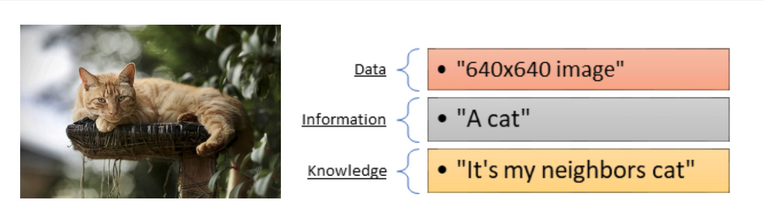
\includegraphics[width=\linewidth]{_fuentes/imagenes/data_vs_info}
      \end{center}
    \column{0.46\textwidth}
      \begin{itemize}
        \item \textbf{Dato}: una imagen 640x640, p\'ixeles en bruto.
        \item \textbf{Informaci\'on}: ``es un gato'' (dato interpretado).
        \item \textbf{Conocimiento}: ``es el gato de mi vecino'' (con contexto).
      \end{itemize}
      \vspace{0.4em}
      El dato no significa nada por s\'i solo: cobra valor cuando lo
      \textbf{interpretamos} y lo ponemos en \textbf{contexto}.
  \end{columns}
\end{frame}

\begin{frame}{La piramide DIKW}
  \begin{center}
  \begin{tikzpicture}[font=\small, every node/.style={align=center}]
    \fill[molTeal]     (-3,0)   -- (3,0)   -- (2.1,1.2) -- (-2.1,1.2) -- cycle;
    \fill[molNaranja]  (-2.1,1.2) -- (2.1,1.2) -- (1.2,2.4) -- (-1.2,2.4) -- cycle;
    \fill[molAmarillo] (-1.2,2.4) -- (1.2,2.4) -- (0.45,3.6) -- (-0.45,3.6) -- cycle;
    \fill[molMorado]   (-0.45,3.6) -- (0.45,3.6) -- (0,4.4) -- cycle;
    \node[white, font=\bfseries] at (0,0.5)  {DATOS};
    \node[white, font=\bfseries] at (0,1.7)  {INFORMACI\'ON};
    \node[font=\bfseries]        at (0,2.85) {CONOCIM.};
    \node[anchor=west] at (3.4,0.5)  {se\~nales, mediciones en bruto};
    \node[anchor=west] at (3.4,1.7)  {datos con significado y relaci\'on};
    \node[anchor=west] at (3.4,2.85) {patrones \'utiles para decidir};
    \node[text=molMorado, font=\bfseries\scriptsize, anchor=west] at (0.8,4.05) {SABIDUR\'IA};
    \node[anchor=west] at (3.4,4.05) {juicio: qu\'e hacer con todo ello};
  \end{tikzpicture}
  \end{center}
\end{frame}

% ======================================================================
\section{Por qu\'e IA y no programaci\'on cl\'asica}

\begin{frame}[fragile]{Dos formas de resolver un problema}
  \begin{center}
  \begin{tikzpicture}[
      box/.style={rounded corners, draw=#1, very thick, fill=#1!10,
                  minimum width=2.3cm, minimum height=0.85cm, align=center,
                  font=\footnotesize\bfseries},
      lbl/.style={font=\scriptsize\itshape, text=molMorado},
      every node/.style={align=center}]
    % Programacion clasica
    \node[lbl] at (3,2.6) {Programaci\'on cl\'asica};
    \node[box=molNaranja] (r1) at (1,1.9) {Reglas};
    \node[box=molNaranja] (d1) at (1,0.8) {Datos};
    \node[box=molTeal]    (p1) at (4.2,1.35) {Programa};
    \node[box=molAmarillo](o1) at (7.2,1.35) {Respuestas};
    \draw[-{Latex[length=2mm]}, thick] (r1) -- (p1);
    \draw[-{Latex[length=2mm]}, thick] (d1) -- (p1);
    \draw[-{Latex[length=2mm]}, thick] (p1) -- (o1);
    % Machine learning
    \node[lbl] at (3,-0.4) {Machine learning};
    \node[box=molNaranja] (d2) at (1,-1.1) {Datos};
    \node[box=molNaranja] (o2) at (1,-2.2) {Respuestas};
    \node[box=molTeal]    (p2) at (4.2,-1.65) {Algoritmo};
    \node[box=molAmarillo](r2) at (7.2,-1.65) {Reglas\\(modelo)};
    \draw[-{Latex[length=2mm]}, thick] (d2) -- (p2);
    \draw[-{Latex[length=2mm]}, thick] (o2) -- (p2);
    \draw[-{Latex[length=2mm]}, thick] (p2) -- (r2);
  \end{tikzpicture}
  \end{center}
  En la programaci\'on cl\'asica escribimos las reglas a mano; en ML el algoritmo
  las \textbf{descubre} a partir de ejemplos.
\end{frame}

\begin{frame}{Hay problemas donde escribir las reglas es imposible}
  \begin{itemize}
    \item Reconocer un gato, una voz o un tumor: \textbf{nadie sabe escribir} las
          reglas exactas, pero tenemos millones de ejemplos.
    \item Juegos con un espacio de b\'usqueda gigantesco:
  \end{itemize}
  \vspace{0.4em}
  \begin{columns}[t]
    \column{0.5\textwidth}
      \begin{block}{Ajedrez}
        \begin{itemize}
          \item Aprox. $10^{47}$ posiciones legales.
          \item \'Arbol de juego $\sim 10^{120}$.
          \item Deep Blue vence a Kasparov en 1997.
        \end{itemize}
      \end{block}
    \column{0.5\textwidth}
      \begin{block}{Go}
        \begin{itemize}
          \item Aprox. $10^{170}$ posiciones.
          \item M\'as que \'atomos en el universo ($\sim 10^{80}$).
          \item AlphaGo vence a Lee Sedol en 2016.
        \end{itemize}
      \end{block}
  \end{columns}
  \vspace{0.3em}
  La fuerza bruta no alcanza: se necesita \textbf{aprender} de datos y experiencia.
\end{frame}

% ======================================================================
\section{Historia: IA, ML y Deep Learning}

\begin{frame}{IA, Machine Learning y Deep Learning}
  \begin{columns}[c]
    \column{0.5\textwidth}
    \begin{center}
    \begin{tikzpicture}
      \fill[molTeal!18, draw=molTeal, very thick] (0,0) circle (3cm);
      \fill[molNaranja!20, draw=molNaranja, very thick] (0,-0.5) circle (2.0cm);
      \fill[molMorado!20, draw=molMorado, very thick] (0,-0.9) circle (1.1cm);
      \node[text=molTeal, font=\bfseries] at (0,2.4) {Inteligencia Artificial};
      \node[text=molNaranja, font=\bfseries] at (0,0.9) {Machine Learning};
      \node[text=molMorado, font=\bfseries\scriptsize, align=center] at (0,-0.9)
        {Deep\\ Learning};
    \end{tikzpicture}
    \end{center}
    \column{0.5\textwidth}
      \begin{itemize}
        \item \textbf{IA}: que las m\'aquinas hagan tareas ``inteligentes''.
        \item \textbf{ML}: subconjunto que \emph{aprende} de datos en vez de
              seguir reglas fijas.
        \item \textbf{DL}: ML con redes neuronales profundas que aprenden
              representaciones por s\'i mismas.
      \end{itemize}
      \vspace{0.3em}
      Cada uno es un subconjunto del anterior.
  \end{columns}
\end{frame}

\begin{frame}[fragile]{Una l\'inea de tiempo de la IA}
  \begin{center}
  \begin{tikzpicture}[font=\scriptsize, every node/.style={align=center}]
    \draw[molTeal, very thick, -{Latex[length=3mm]}] (0,0) -- (12,0);
    \foreach \x/\y/\a in {
        0/1950/Test de Turing,
        2/1956/Dartmouth:\\ nace ``IA'',
        4/1980/Sistemas\\ expertos,
        6/1997/Deep Blue\\ vence ajedrez,
        8/2012/ImageNet:\\ AlexNet (DL),
        10/2016/AlphaGo\\ vence Go,
        12/2017/Transformers\\ -> LLMs} {
      \fill[molNaranja] (\x,0) circle (2.2pt);
      \node[text=molMorado, font=\scriptsize\bfseries] at (\x,-0.45) {\y};
      \node[anchor=south, text width=1.9cm] at (\x,0.12) {\a};
    }
  \end{tikzpicture}
  \end{center}
  \vspace{0.6em}
  Dos ``inviernos de la IA'' (1974--80 y 1987--93) frenaron el campo cuando las
  promesas superaron a los \textbf{datos} y al \textbf{c\'omputo} disponibles.
\end{frame}

\begin{frame}{2012: el a\~no en que los datos cambiaron todo}
  \begin{columns}[c]
    \column{0.46\textwidth}
      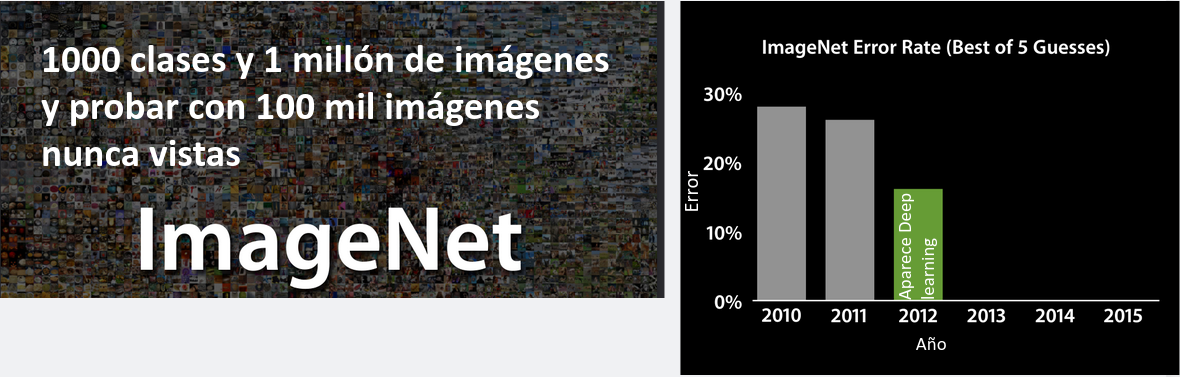
\includegraphics[width=\linewidth]{_fuentes/imagenes/imagenet_1}
    \column{0.54\textwidth}
      \textbf{ImageNet}: 1000 clases y m\'as de 1 mill\'on de im\'agenes
      etiquetadas.
      \begin{itemize}
        \item En 2012 AlexNet (red profunda + GPUs) baj\'o dr\'asticamente el error.
        \item Deton\'o la era del \textbf{deep learning}.
        \item Sin ese \textbf{dataset masivo} no habr\'ia ocurrido.
      \end{itemize}
      Moraleja: el avance vino tanto de los \textbf{datos} como del algoritmo.
  \end{columns}
\end{frame}

% ======================================================================
\section{ML vs Deep Learning}

\begin{frame}[fragile]{Machine Learning cl\'asico vs Deep Learning}
  \begin{center}
  \begin{tikzpicture}[
      stg/.style={rounded corners, draw=#1, very thick, fill=#1!12,
                  minimum height=0.9cm, align=center, font=\scriptsize\bfseries},
      every node/.style={align=center}]
    % ML clasico
    \node[font=\footnotesize\bfseries, text=molMorado] at (3.6,3.0) {ML cl\'asico};
    \node[stg=molTeal, minimum width=1.7cm]    (i1) at (0,2.0) {Entrada};
    \node[stg=molNaranja, minimum width=2.4cm] (f1) at (2.8,2.0) {Extracci\'on de\\ atributos (manual)};
    \node[stg=molMorado, minimum width=1.9cm]  (m1) at (5.6,2.0) {Modelo};
    \node[stg=molAmarillo, minimum width=1.6cm](o1) at (8.0,2.0) {Salida};
    \draw[-{Latex[length=2mm]},thick] (i1)--(f1); \draw[-{Latex[length=2mm]},thick] (f1)--(m1); \draw[-{Latex[length=2mm]},thick] (m1)--(o1);
    \node[text=molNaranja, font=\scriptsize] at (2.8,1.2) {lo dise\~na el humano};
    % Deep learning
    \node[font=\footnotesize\bfseries, text=molMorado] at (3.6,-0.3) {Deep Learning};
    \node[stg=molTeal, minimum width=1.7cm]   (i2) at (0,-1.3) {Entrada};
    \node[stg=molMorado, minimum width=4.3cm] (m2) at (4.2,-1.3) {Red neuronal profunda:\\ aprende atributos + decide};
    \node[stg=molAmarillo, minimum width=1.6cm](o2) at (8.0,-1.3) {Salida};
    \draw[-{Latex[length=2mm]},thick] (i2)--(m2); \draw[-{Latex[length=2mm]},thick] (m2)--(o2);
    \node[text=molMorado, font=\scriptsize] at (4.2,-2.1) {lo aprende la red, extremo a extremo};
  \end{tikzpicture}
  \end{center}
  El DL evita el dise\~no manual de atributos, pero a cambio exige
  \textbf{muchos m\'as datos} y c\'omputo.
\end{frame}

\begin{frame}{Cu\'ando usar cada uno}
  \begin{columns}[t]
    \column{0.5\textwidth}
      \begin{block}{ML cl\'asico}
        \begin{itemize}
          \item Datos tabulares, pocos ejemplos.
          \item R\'apido e interpretable.
          \item Ej.: \'arboles, SVM, regresi\'on.
        \end{itemize}
      \end{block}
    \column{0.5\textwidth}
      \begin{block}{Deep Learning}
        \begin{itemize}
          \item Im\'agenes, voz, texto, video.
          \item Muchos datos y GPUs.
          \item Ej.: CNN, RNN, Transformers.
        \end{itemize}
      \end{block}
  \end{columns}
  \vspace{0.5em}
  No siempre ``m\'as profundo es mejor'': con datos peque\~nos el ML cl\'asico
  suele ganar.
\end{frame}

% ======================================================================
\section{Taxonom\'ia del Machine Learning}

\begin{frame}[fragile]{Los cuatro grandes tipos de aprendizaje}
  \begin{center}
  \begin{tikzpicture}[
      font=\scriptsize,
      root/.style={rounded corners, draw=molTeal, very thick, fill=molTeal!12,
                   font=\footnotesize\bfseries, minimum width=2.6cm, minimum height=0.8cm},
      cat/.style={rounded corners, draw=#1, very thick, fill=#1!15,
                  font=\scriptsize\bfseries, align=center, minimum width=2.3cm,
                  minimum height=0.85cm},
      ex/.style={align=center, font=\scriptsize, text width=2.6cm},
      every node/.style={align=center}]
    \node[root] (ml) at (5.5,4.2) {Machine Learning};
    \node[cat=molMorado]  (sl)  at (0.6,2.6) {Supervisado};
    \node[cat=molNaranja] (ssl) at (3.9,2.6) {Semi-\\supervisado};
    \node[cat=molAmarillo](ul)  at (7.1,2.6) {No\\supervisado};
    \node[cat=molAzul]    (rl)  at (10.4,2.6) {Por refuerzo};
    \draw[molTeal, thick] (ml) -- (sl);
    \draw[molTeal, thick] (ml) -- (ssl);
    \draw[molTeal, thick] (ml) -- (ul);
    \draw[molTeal, thick] (ml) -- (rl);
    \node[ex] at (0.6,1.2) {datos etiquetados\\ \textit{clasificaci\'on,\\ regresi\'on}\\ spam, precios};
    \node[ex] at (3.9,1.2) {pocos con etiqueta\\ + muchos sin ella\\ \textit{web, im\'agenes\\ m\'edicas}};
    \node[ex] at (7.1,1.2) {sin etiquetas\\ \textit{clustering,\\ reducci\'on dim.}\\ segmentar clientes};
    \node[ex] at (10.4,1.2) {premio/castigo\\ \textit{agente que act\'ua}\\ AlphaGo, rob\'otica};
  \end{tikzpicture}
  \end{center}
  \vspace{0.2em}
  El \textbf{etiquetado} de datos es caro: por eso el semi-supervisado y el
  auto-supervisado (base de los LLM) son tan importantes hoy.
\end{frame}

% ======================================================================
\section{Premios: Turing y Nobel}

\begin{frame}{El campo en su punto m\'as alto: dos grandes premios}
  \begin{columns}[t]
    \column{0.5\textwidth}
      \begin{block}{Premio Turing 2018}
        \small
        El ``Nobel de la computaci\'on'' a \textbf{Yoshua Bengio},
        \textbf{Geoffrey Hinton} y \textbf{Yann LeCun} por los avances
        conceptuales y de ingenier\'ia que hicieron del \textbf{deep learning}
        un componente cr\'itico de la computaci\'on.
      \end{block}
    \column{0.5\textwidth}
      \begin{block}{Premio Nobel 2024}
        \small
        \textbf{F\'isica}: J. Hopfield y G. Hinton, por descubrimientos que
        permiten el \textbf{aprendizaje con redes neuronales artificiales}.\\[0.3em]
        \textbf{Qu\'imica}: D. Hassabis y J. Jumper (AlphaFold), por
        \textbf{predecir la estructura de las prote\'inas} con IA.
      \end{block}
  \end{columns}
  \vspace{0.4em}
  Hinton aparece en ambos: las redes neuronales pasaron de curiosidad a motor de
  la ciencia.
\end{frame}

\begin{frame}{Un nuevo paradigma para hacer ciencia}
  \begin{center}
    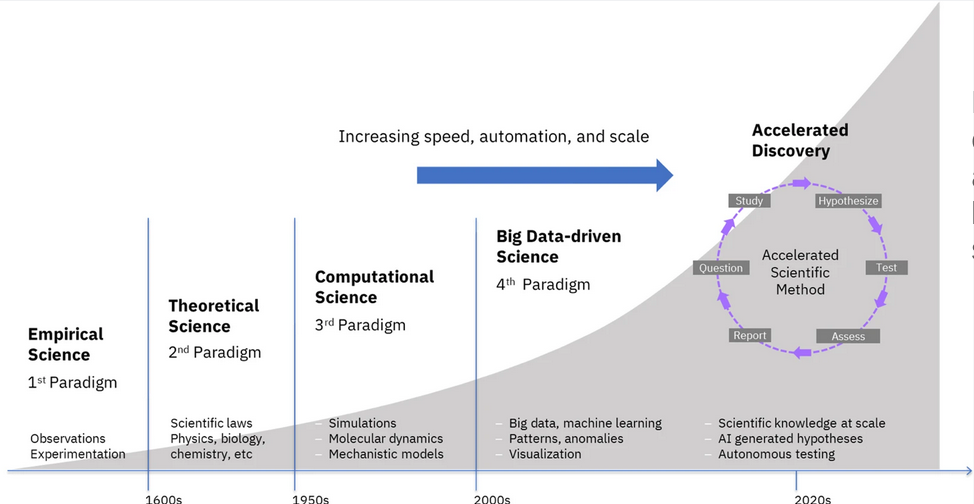
\includegraphics[width=0.8\linewidth]{_fuentes/imagenes/paradigmas_ciencia}
  \end{center}
  \vspace{-0.2em}
  De la ciencia emp\'irica a la ciencia \textbf{guiada por datos} (4to paradigma):
  la IA acelera el descubrimiento (AlphaFold es el mejor ejemplo).
\end{frame}

% ======================================================================
\section{Retos actuales de los datos}

\begin{frame}[t]{La IA ya alcanza o supera al humano en muchas tareas}
  \begin{center}
    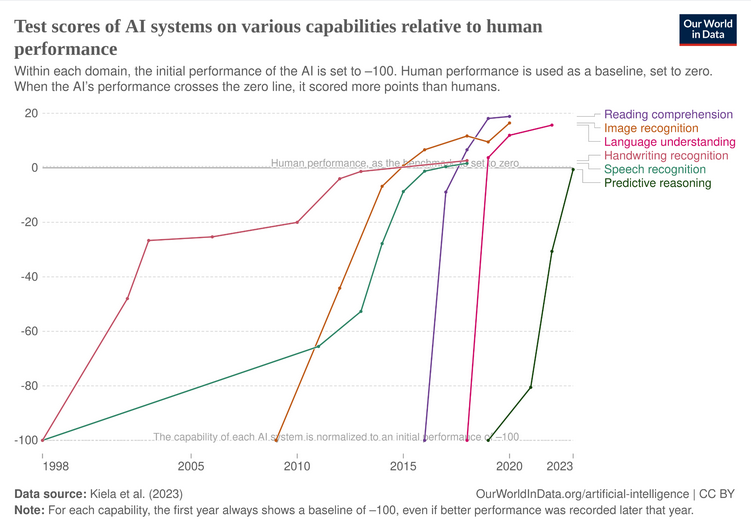
\includegraphics[width=0.56\linewidth]{_fuentes/imagenes/timeline_ai_humano}\\[0.4em]
    \small Cada salto fue posible por \textbf{m\'as y mejores datos}.
  \end{center}
\end{frame}

\begin{frame}{LLMs y agentes: hambre de datos a gran escala}
  \begin{itemize}
    \item Los \textbf{LLM} se entrenan con billones de palabras (gran parte de la
          web) y miles de millones de par\'ametros.
    \item Los \textbf{agentes} encadenan modelos con herramientas y memoria:
          generan y consumen a\'un m\'as datos.
    \item Retos: \textbf{volumen} (almacenar y mover petabytes), \textbf{calidad}
          y sesgos, \textbf{licencias} y privacidad, y datos \textbf{frescos}.
    \item Se discute incluso un posible ``agotamiento'' de datos p\'ublicos de
          alta calidad y el uso de \textbf{datos sint\'eticos}.
  \end{itemize}
\end{frame}

\begin{frame}{De la gesti\'on tradicional a datos ``AI-ready''}
  \begin{center}
    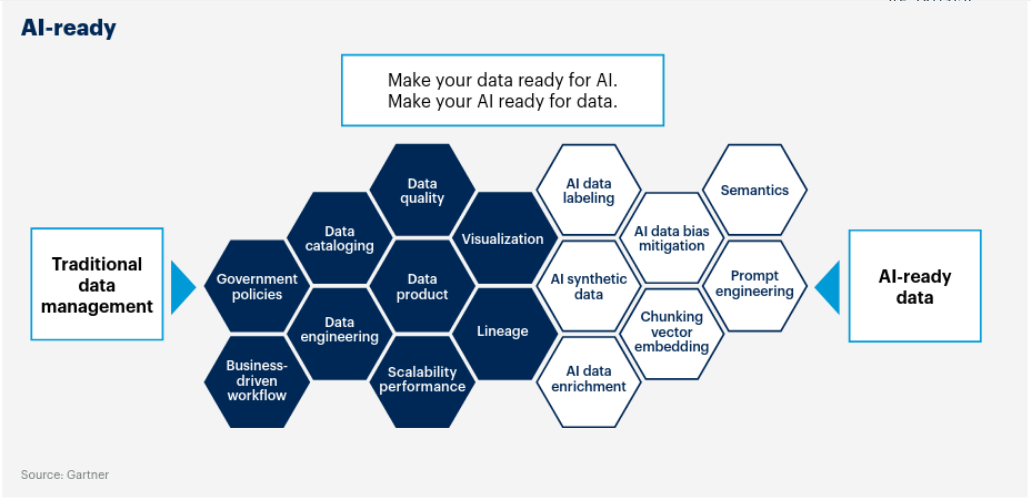
\includegraphics[width=0.78\linewidth]{_fuentes/imagenes/human_machinedata}
  \end{center}
  \vspace{-0.2em}
  {\scriptsize\color{gray}Fuente: Gartner.}\\
  Preparar datos para IA agrega etapas nuevas: etiquetado, \emph{embeddings},
  \emph{chunking}, mitigaci\'on de sesgos y \emph{prompt engineering}.
\end{frame}

% ======================================================================
\section{Resumen}

\begin{frame}{Takeaways}
  \begin{itemize}
    \item La IA se sostiene en tres pilares: \textbf{datos, infraestructura y
          personas}; los datos son hoy el factor diferenciador.
    \item \textbf{Dato} no es \textbf{informaci\'on}: el valor surge al
          interpretar y contextualizar.
    \item Hay problemas (ajedrez, Go, visi\'on) donde \textbf{no se pueden
          escribir las reglas}: hay que aprenderlas de datos.
    \item \textbf{IA $\supset$ ML $\supset$ DL}; el DL despeg\'o en 2012 gracias a
          ImageNet y las GPUs.
    \item Premios \textbf{Turing 2018} y \textbf{Nobel 2024} consagraron a las
          redes neuronales.
    \item El futuro (LLMs, agentes) depende de datos a \textbf{gran escala} y de
          calidad: ese es el reto del diplomado.
  \end{itemize}
\end{frame}

\begin{frame}[plain]
  \molinaBanner
  \vfill
  \begin{center}
    {\color{molMorado}\Large\bfseries Gracias}\\[0.4em]
    {\color{molTeal} Siguiente: el lenguaje de los datos en la pr\'actica}
  \end{center}
  \vfill\vspace{1.0cm}
  \molinaLogos
\end{frame}

\end{document}
